\documentclass{math}

\usepackage{tikz}

\title{University Physics 2}
\author{Alvin Lin}
\date{January 2018 - May 2018}

\begin{document}

\maketitle

\section*{Electric Fields}
We know positive charges feel repulsive forces from other positive charges. If
we take a test charge and place it near an object of interest, how it would
experience a force is the direction of the electric field, also known as the
E-field. We define it as:
\[ \vec{E} = \frac{\vec{F_{\circ}}}{q_{\circ}} \]
where \( \vec{F_{\circ}} \) is the force on the test charge, \( q_{\circ} \)
is the test charge, and \( \vec{E} \) is the electric field from some charge
distribution. Usually, we will represent this in the form:
\[ \vec{F} = q\vec{E} \]
This allows us to calculate the force \( \vec{F} \) for some charge \( q \)
exerted by an external electric field \( \vec{E} \). For a point charge, we
calculate the field with:
\[ \vec{E_{pc}} = \frac{Kq\hat{r}}{r^2} \]
This is the same as Coulomb's Law but is measured in Newtons per Coulomb. This
is due to the fact that there is no second charge from the observation charge.
The field lines point away from positive charges and towards negative charges.
\begin{center}
  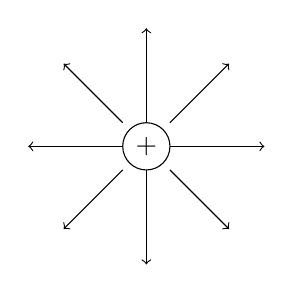
\begin{tikzpicture}[scale=1.5]
    \draw (0,0) circle (0.2cm) node {+};
    \draw[->] (0.2,0) -- (1,0);
    \draw[->] (0.2,0.2) -- (0.7,0.7);
    \draw[->] (0,0.2) -- (0,1);
    \draw[->] (-0.2,0.2) -- (-0.7,0.7);
    \draw[->] (-0.2,0) -- (-1,0);
    \draw[->] (-0.2,-0.2) -- (-0.7,-0.7);
    \draw[->] (0,-0.2) -- (0,-1);
    \draw[->] (0.2,-0.2) -- (0.7,-0.7);
  \end{tikzpicture}
  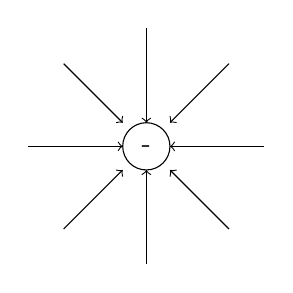
\begin{tikzpicture}[scale=1.5]
    \draw (0,0) circle (0.2cm) node {-};
    \draw[<-] (0.2,0) -- (1,0);
    \draw[<-] (0.2,0.2) -- (0.7,0.7);
    \draw[<-] (0,0.2) -- (0,1);
    \draw[<-] (-0.2,0.2) -- (-0.7,0.7);
    \draw[<-] (-0.2,0) -- (-1,0);
    \draw[<-] (-0.2,-0.2) -- (-0.7,-0.7);
    \draw[<-] (0,-0.2) -- (0,-1);
    \draw[<-] (0.2,-0.2) -- (0.7,-0.7);
  \end{tikzpicture}
\end{center}

\subsection*{Electric Dipoles: Off-Axis Field}
\begin{center}
  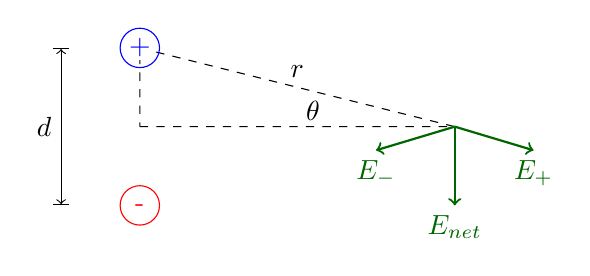
\begin{tikzpicture}
    \draw[|<->|] (-1,1) -- (-1,-1) node[pos=0.5,left] {\( d \)};
    \draw[dashed] (0,0) -- (4,0) -- node[pos=0.5,above] {\( r \)} (0,1) --
      cycle;
    \node at (2.2,0.2) {\( \theta \)};
    \draw[blue] (0,1) circle (0.25cm) node[fill=white,inner sep=0.04cm] {+};
    \draw[red] (0,-1) circle (0.25cm) node[fill=white,inner sep=0.04cm] {-};
    \draw[->,thick,black!60!green] (4,0) -- (3,-0.3) node[below] {\( E_{-} \)};
    \draw[->,thick,black!60!green] (4,0) -- (5,-0.3) node[below] {\( E_{+} \)};
    \draw[->,thick,black!60!green] (4,0) -- (4,-1) node[below] {\( E_{net} \)};
  \end{tikzpicture}
\end{center}
The x-components of the fields cancel.
\begin{align*}
  E_{+} &= \frac{kq}{r^2} \\
  E_{+,y} &= E_{+}\sin\theta = \frac{kq\sin\theta}{r^2}
\end{align*}
In the case where \( \frac{d}{x} << 1 \):
\begin{align*}
  \left(\frac{d}{x}\right)^2 &\approx 0 \quad
    \sin\theta = \frac{\frac{d}{2}}{r} \quad
    r = \sqrt{x^2+\bigg(\frac{d}{2}\bigg)^2} \\
  E_{+,y} &= \frac{kq\sin\theta}{r^2}
    = \frac{kq}{r^2}\frac{\frac{d}{2}}{r}
    = \frac{1}{2}\frac{kqd}{r^3} \\
  &= \frac{1}{2}\frac{kqd}{\bigg(\sqrt{x^2+\frac{d^2}{4}}\bigg)^3} \\
  &= \frac{1}{2}kqd\bigg[x^2+\frac{d^2}{4}\bigg]^{-\frac{3}{2}} \\
  &= \frac{1}{2}kqdx^{-3}\bigg[1+\frac{d^2}{4x^2}\bigg]^{-\frac{3}{2}} \\
  &\approx \frac{1}{2}kqdx^{-3}\bigg(1+0\bigg)^{-\frac{3}{2}} \\
  &\approx \frac{kqd}{2x^3} \\
  E_{net} &= 2E_{+,y} = \frac{kqd}{x^3}
\end{align*}

\subsection*{Electric Dipoles: On-Axis Field}
\begin{center}
  \begin{tikzpicture}
    \draw[blue] (0,1) circle (0.25cm) node {+};
    \draw[red] (0,-1) circle (0.25cm) node {-};
    \draw[|<->|] (-1,1) -- (-1,-1) node[pos=0.5,left] {\( d \)};
    \draw[|<->|] (-1,1) -- (-1,4) node[pos=0.5,left] {\( r_{+} \)};
    \draw[fill,black!60!green] (0,4) circle (0.05cm) node[above] {point};
    \draw[|<->|] (1,0) -- (1,4) node[pos=0.5,right] {\( z \)};
  \end{tikzpicture}
\end{center}
In the case where \( d << x \), we can use the binomial expansion:
\begin{align*}
  (1+\epsilon)^n &\approx 1+n\epsilon \\
  E_{+} &= \frac{kq}{r_{+}^2} = \frac{kq}{(z-\frac{d}{2})^2} \\
  &= kqz^{-2}(1-\frac{d}{2z})^{-2} \\
  &\approx kqz^{-2}\bigg(1+(-2)(\frac{-d}{2n})\bigg) \\
  &\approx kqz^{-2}(1+\frac{d}{z}) \\
  E_{-} &= \frac{kq}{(r_{+}+d)^2} = \frac{kq}{(z+\frac{d}{2})^2} \\
  &= kqz^{-2}(1+\frac{d}{2z})^{-2} \\
  &\approx kqz^{-2}(1-\frac{d}{z}) \\
  E_{net} &= E_{+}-E_{-} \\
  &= (\frac{kq}{z^2}+\frac{kqd}{z^3})-(\frac{kq}{z^2}-\frac{kqd}{z^3}) \\
  &= \frac{2kqd}{z^3}
\end{align*}
Note that for a point charge, \( E\sim\frac{1}{r^2} \), and for a dipole
\( E\sim\frac{1}{r^3} \).

\subsection*{Dipole Moment}
\begin{center}
  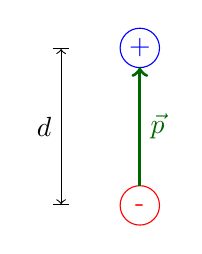
\begin{tikzpicture}
    \draw[blue] (0,1) circle (0.25cm) node {+};
    \draw[red] (0,-1) circle (0.25cm) node {-};
    \draw[|<->|] (-1,1) -- (-1,-1) node[pos=0.5,left] {\( d \)};
    \draw[->,black!60!green,very thick] (0,-0.75) -- (0,0.75)
      node[pos=0.5,right] {\( \vec{p} \)};
  \end{tikzpicture}
\end{center}
In this diagram, \( \vec{p} \) is the dipole moment. It points from negative to
positive and has a magnitude of \( qd \). For the on-axis field:
\[ \vec{E} = \frac{2k\vec{p}}{z^3} \quad \vec{p} = qd\j \]
For the off-axis field:
\[ \vec{E} = \frac{-k\vec{p}}{z^3} \quad \vec{p} = qd\j \]

\subsection*{Dipoles in Electric Fields}
\begin{center}
  \begin{tikzpicture}[scale=2]
    \node[black!60!green,right] at (4,2) {\( E \)};
    \foreach \y in {0,1,2} {
      \draw[->,black!60!green] (0,\y) -- (4,\y);
    }
    \draw[blue] (2,1.5) circle (0.1cm) node {+};
    \draw[red] (1,0.5) circle (0.1cm) node {-};
    \draw[dashed] (1.1,0.6) -- (1.9,1.4) node[pos=0.65,right] {\( \theta \)};
    \draw[|<->|] (0.75,0.75) -- (1.75,1.75) node[pos=0.5,above] {\( d \)};
  \end{tikzpicture}
\end{center}
\begin{align*}
  \vec{F} &= q\vec{E}+(-q\vec{E}) = 0 \\
  |\tau| &= dq\vec{E}\sin\theta = \vec{p}\vec{E}\sin\theta \\
  \vec{\tau} &= \vec{p}\times\vec{E}
\end{align*}

\subsection*{Electric Fields of Solid Objects}
Strategy for calculating the electric field of a solid object:
\begin{enumerate}
  \item Draw a diagram: draw the axes, place the charge, draw \( \diff{q} \),
  and any distances (\( r,x,\theta,\dots \)).
  \item Calculate the charge density \( \lambda \). If it is uniform, then
  \( \lambda = \frac{Q}{L} \). Otherwise, it is a function \( \lambda(r) \) and
  we need to integrate.
  \item Figure out \( \diff{q} \). \( \diff{q} = \lambda\diff{s} \). For a line
  \( \diff{s} = \diff{x} \). For an arc, \( \diff{s} = r\diff{\theta} \).
  \item Find \( |\diff{E}| \)
  \[ \diff{E} = \frac{k\diff{q}}{r^2} \]
  \item Find the components.
  \[ \diff{E_x} = |\diff{E}|\cos\theta \]
  \[ \diff{E_y} = |\diff{E}|\sin\theta \]
  Note that this depends on whether or not \( \theta \) is from the horizontal.
  \item Get the limits of integration from the diagram.
  \item Check for symmetries to see if any integrals are zero.
  \item Integrate:
  \[ E_x = \int\diff{E_x} \]
\end{enumerate}

\subsubsection*{Example}
\begin{center}
  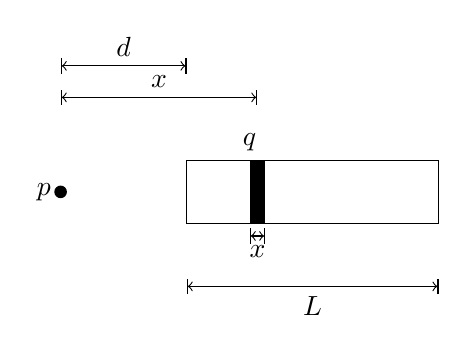
\begin{tikzpicture}[scale=0.8]
    \draw (0,0) -- (4,0) -- (4,1) -- (0,1) -- cycle;
    \fill (-2,0.5) circle (0.1cm) node[left] {\( p \)};
    \fill (1,0) -- (1.25,0) -- (1.25,1) -- (1,1) node[above] {\( \diff{q} \)};
    \draw[|<->|] (-2,2.5) -- (0,2.5) node[pos=0.5,above] {\( d \)};
    \draw[|<->|] (-2,2) -- (1.125,2) node[pos=0.5,above] {\( x \)};
    \draw[|<->|] (1,-0.2) -- (1.25,-0.2) node[pos=0.5,below] {\( \diff{x} \)};
    \draw[|<->|] (0,-1) -- (4,-1) node[pos=0.5,below] {\( L \)};
  \end{tikzpicture}
\end{center}
\begin{align*}
  E &= \frac{kQ}{r^2} \quad \diff{E} = \frac{k\diff{q}}{r^2} \\
  r &= x \quad
    \lambda = \frac{Q}{L} \quad
    \diff{q} = \lambda\diff{s} = \frac{Q}{L}\diff{x} \\
  |E| &= \int_{d}^{d+L}\frac{kQ}{Lx^2}\diff{x}
    = \frac{kQ}{L}\bigg[-\frac{1}{x}\bigg]_{d}^{d+L} \\
  &= \frac{kQ}{d(d+L)}
\end{align*}
Let's consider the field where the point is very far away from the rod.
\[ d >> L \Rightarrow \frac{L}{d} << 1 \Rightarrow \frac{L}{d}\sim 0 \]
In this case, where the point is very far away, the field of the rod looks like
the field of a point charge:
\[ |E| = \frac{kQ}{(d(d+L))} = \frac{kQ}{d^2(1+\frac{L}{d})} \sim
  \frac{kQ}{d^2} \]

\subsubsection*{Example}
\begin{center}
  \begin{tikzpicture}
    \draw (-4,0) -- (4,0) -- (4,0.8) -- (-4,0.8) -- cycle;
    \fill (0,3) circle (0.1cm) node[above] {\( p \)};
    \fill (-2.25,0) -- (-2,0) -- (-2,0.8) -- (-2.25,0.8)
      node[above] {\( \diff{q} \)};
    \draw[dashed] (0,0.4) -- node[pos=0.5,below] {\( x \)} (-2.125,0.4)
      -- (0,3) node[pos=0.5,above] {\( r \)}
      -- (0,0.4) node[pos=0.5,right] {\( h \)};
    \draw[|<->|] (-2.25,-0.2) -- (-2,-0.2) node[pos=0.5,below] {\( \diff{x} \)};
    \draw[|<->|] (-4,-1) -- (4,-1) node[pos=0.5,below] {\( L \)};
  \end{tikzpicture}
\end{center}
By symmetry, we can see that the field in the x-direction cancels out, but we
will solve it for completeness. Our known values are as follows:
\begin{align*}
  E &= \frac{kQ}{r^2} \quad \diff{E} = \frac{k\diff{q}}{r^2} \\
  r^2 &= x^2+h^2 \quad \lambda = \frac{Q}{L} \quad \\
  \diff{q} &= \lambda\diff{s} = \frac{Q}{L}\diff{x} \\
  \cos\theta &= \frac{x}{h} \\
  \sin\theta &= \frac{h}{r} = \frac{h}{\sqrt{x^2+h^2}}
\end{align*}
Since the point is on a different axis than the rod, we have to separate the
electric field into components.
\begin{align*}
  \diff{E_x} &= \diff{E}\cos\theta \\
  &= \frac{kQ}{Lr^2}\frac{x}{r}\diff{x} \\
  &= \frac{kQ}{L}\frac{x}{(x^2+h^2)^{\frac{3}{2}}}\diff{x} \\
  E_x &= \int_{-\frac{L}{2}}^{\frac{L}{2}}
    \frac{kQ}{L}\frac{x}{(x^2+h^2)^{\frac{3}{2}}}\diff{x} = 0 \\
  \diff{E_y} &= \diff{E}\sin\theta \\
  &= \frac{kQ}{Lr^2}\frac{h}{r}\diff{x} \\
  &= \frac{kQh}{L}\frac{1}{(h^2+x^2)^{\frac{3}{2}}}\diff{x} \\
  E_y &= \int_{-\frac{L}{2}}^{\frac{L}{2}}
    \frac{kQh}{L}\frac{1}{(x^2+h^2)^{\frac{3}{2}}}\diff{x} \\
  &= \frac{kQ}{h\sqrt{h^2+\frac{L^2}{4}}}
\end{align*}
Since the field in the x-direction cancels out:
\[ |\vec{E}| = E_y = \frac{kQ}{h\sqrt{h^2+\frac{L^2}{4}}}\j \]
Let's consider two limits: suppose the point is very far away from the rod:
\[ h >> L \Rightarrow \frac{L}{h} << 1 \Rightarrow \frac{L}{h}\sim 0 \]
Like before, the field of the rod looks like that of a point charge:
\[ |E| = \frac{kQ}{h\sqrt{h^2+\frac{L^2}{4}}} =
  \frac{kQ}{h^2(1+\frac{L^2}{4h^2})} \sim \frac{kQ}{h^2} \]
Let's consider now a very long rod (or having the point inside the rod):
\[ L >> h \Rightarrow \frac{h}{L} \sim 0 \]
This gives us a very interesting result:
\[ |E| \]

\subsubsection*{Example}
\begin{center}
  \begin{tikzpicture}
    \draw (4,1) -- (0,1) -- (0,0) -- (4,0);
    \fill (1,0) -- (1.25,0) -- (1.25,1) -- (1,1);
    \fill (-2,0.5) circle (0.1cm) node[above] {\( p \)};
    \draw[|<->|] (-2,2) -- (0,2) node[pos=0.5,above] {\( d \)};
    \draw[|<->|] (-2,-1) -- (1,-1) node[pos=0.5,below] {\( x \)};
    \draw[->] (4,0.5) -- (5,0.5) node[right] {to \( \infty \)};
  \end{tikzpicture}
\end{center}
In this example, there is an infinite line of charge along the x-axis with a
non-uniform charge density of \( \lambda = \beta x^{-3} \). The units of
\( \beta \) are given in Coulomb \( \cdot \) meters squared.
\begin{align*}
  \diff{q} &= \lambda\diff{x} \\
  &= \frac{\beta}{x^3}\diff{x} \\
  Q &= \int_{d}^{\infty}\frac{\beta}{x^3}\diff{x} \\
  &= \bigg[\beta\frac{-1}{2}x^{-2}\bigg]_{d}^{\infty} \\
  &= -\frac{\beta}{2}\bigg(\frac{1}{\infty^2}-\frac{1}{d^2}\bigg) \\
  &= \frac{\beta}{2d^2} \\
\end{align*}
\begin{align*}
  \diff{E} &= \frac{k\diff{q}}{r^2} \\
  &= \frac{k\beta}{x^5}\diff{x} \\
  |E| &= \int_{d}^{\infty}\diff{E} \\
  &= k\beta\bigg[\frac{-1}{4}x^{-4}\bigg]_{d}^{\infty} \\
  &= -\frac{k\beta}{4}\bigg(\frac{1}{\infty^4}-\frac{1}{d^4}\bigg) \\
  &= \frac{k\beta}{4d^4}
\end{align*}
The direction of this field is to the left from the point charge \( p \).

\begin{center}
  You can find all my notes at \url{http://omgimanerd.tech/notes}. If you have
  any questions, comments, or concerns, please contact me at
  alvin@omgimanerd.tech
\end{center}

\end{document}
